\documentclass[tikz,border=14pt]{standalone}

\usepackage{tikz}
\usetikzlibrary{
  shapes.geometric, shapes.misc,
  arrows.meta, arrows,
  positioning, fit, calc,
  backgrounds, shadows
}
\usepackage{amsmath,amssymb}
\usepackage{xcolor}
\usepackage[T1]{fontenc}

%% ── Color Palette ────────────────────────────────────────────
\definecolor{navyblue}{RGB}{20,60,120}
\definecolor{coralred}{RGB}{210,80,70}
\definecolor{mintgreen}{RGB}{60,160,110}
\definecolor{amber}{RGB}{200,140,30}
\definecolor{lavender}{RGB}{120,90,170}
\definecolor{boxblue}{RGB}{210,225,245}
\definecolor{boxred}{RGB}{245,215,215}
\definecolor{boxorange}{RGB}{255,232,205}
\definecolor{boxgray}{RGB}{228,228,228}
\definecolor{boxgreen}{RGB}{200,235,210}
\definecolor{boxpurple}{RGB}{228,215,242}
\definecolor{cDark}{RGB}{40,60,100}
\definecolor{fusioncolor}{RGB}{200,80,20}
\definecolor{rlblue}{RGB}{30,90,160}
\definecolor{rlgreen}{RGB}{20,140,60}
\definecolor{rlred}{RGB}{180,40,40}
\definecolor{memorycol}{RGB}{200,180,240}
\definecolor{qnetcol}{RGB}{170,210,250}
\definecolor{actioncol}{RGB}{245,220,170}
\definecolor{nlpcol}{RGB}{200,240,200}
\definecolor{rlpolicy}{RGB}{255,235,200}
\definecolor{rlpolicyborder}{RGB}{180,100,20}
% New RL injection colors
\definecolor{rlAudio}{RGB}{255,220,200}
\definecolor{rlVideo}{RGB}{220,245,220}
\definecolor{rlText}{RGB}{220,230,255}
\definecolor{rlFusion}{RGB}{245,220,245}
\definecolor{rlRobot}{RGB}{240,250,255}

%% ── Node Styles ─────────────────────────────────────────────
\tikzset{
  basebox/.style={rectangle,rounded corners=5pt,draw=black!50,align=center,font=\small},
  inputnode/.style={basebox,fill=cDark,text=white,minimum width=3.0cm,minimum height=1.1cm,font=\small\bfseries},
  encnode/.style={basebox,fill=boxblue,draw=navyblue!70,minimum width=3.0cm,minimum height=1.0cm,thick},
  projnode/.style={basebox,fill=boxorange,draw=amber!80,minimum width=3.0cm,minimum height=1.0cm,thick},
  retnode/.style={basebox,fill=boxgreen,draw=mintgreen!80,minimum width=3.0cm,minimum height=1.0cm,thick},
  gennode/.style={basebox,fill=boxred,draw=coralred!80,minimum width=3.0cm,minimum height=1.0cm,thick},
  outnode/.style={basebox,fill=boxpurple,draw=lavender!80,minimum width=3.0cm,minimum height=1.0cm},
  fusnode/.style={basebox,fill=fusioncolor!15,draw=fusioncolor!70,minimum width=3.2cm,minimum height=1.0cm,thick},
  decnode/.style={diamond,draw=amber!90,fill=yellow!25,aspect=2.8,align=center,font=\small\bfseries,minimum width=3.0cm,minimum height=1.2cm},
  datanode/.style={basebox,fill=boxgray,draw=black!40,minimum width=2.8cm,minimum height=0.9cm,font=\small},
  lossnode/.style={basebox,fill=boxorange,draw=amber!80,minimum width=3.0cm,minimum height=1.0cm},
  qnetnode/.style={basebox,fill=qnetcol,draw=rlblue,minimum width=3.0cm,minimum height=1.2cm,thick},
  memnode/.style={basebox,fill=memorycol,draw=lavender,minimum width=3.0cm,minimum height=1.0cm},
  robotnode/.style={basebox,fill=actioncol,draw=amber,minimum width=3.0cm,minimum height=1.0cm,thick},
  nlpnode/.style={basebox,fill=nlpcol,draw=mintgreen,minimum width=3.0cm,minimum height=1.0cm},
  % New: RL policy injection nodes (orange-bordered, distinguished)
  rlpnode/.style={basebox,fill=rlpolicy,draw=rlpolicyborder,minimum width=3.2cm,minimum height=1.1cm,thick,
                  font=\small\bfseries},
  arr/.style={->,>=Stealth,thick,color=black!70},
  thickarr/.style={->,>=Stealth,very thick,color=cDark},
  redarr/.style={->,>=Stealth,thick,color=coralred!80},
  greenarr/.style={->,>=Stealth,thick,color=mintgreen!80},
  bluearr/.style={->,>=Stealth,thick,color=rlblue},
  dasharr/.style={->,>=Stealth,thick,dashed,color=gray!70},
  ambarr/.style={->,>=Stealth,thick,dashed,color=amber!90},
  rlarr/.style={->,>=Stealth,very thick,color=rlpolicyborder},        % RL reward/feedback arrows
  rldasharr/.style={->,>=Stealth,thick,dashed,color=rlpolicyborder}   % RL dashed
}

\newcommand{\R}{\mathbb{R}}
\newcommand{\Sph}{\mathbb{S}}

\begin{document}
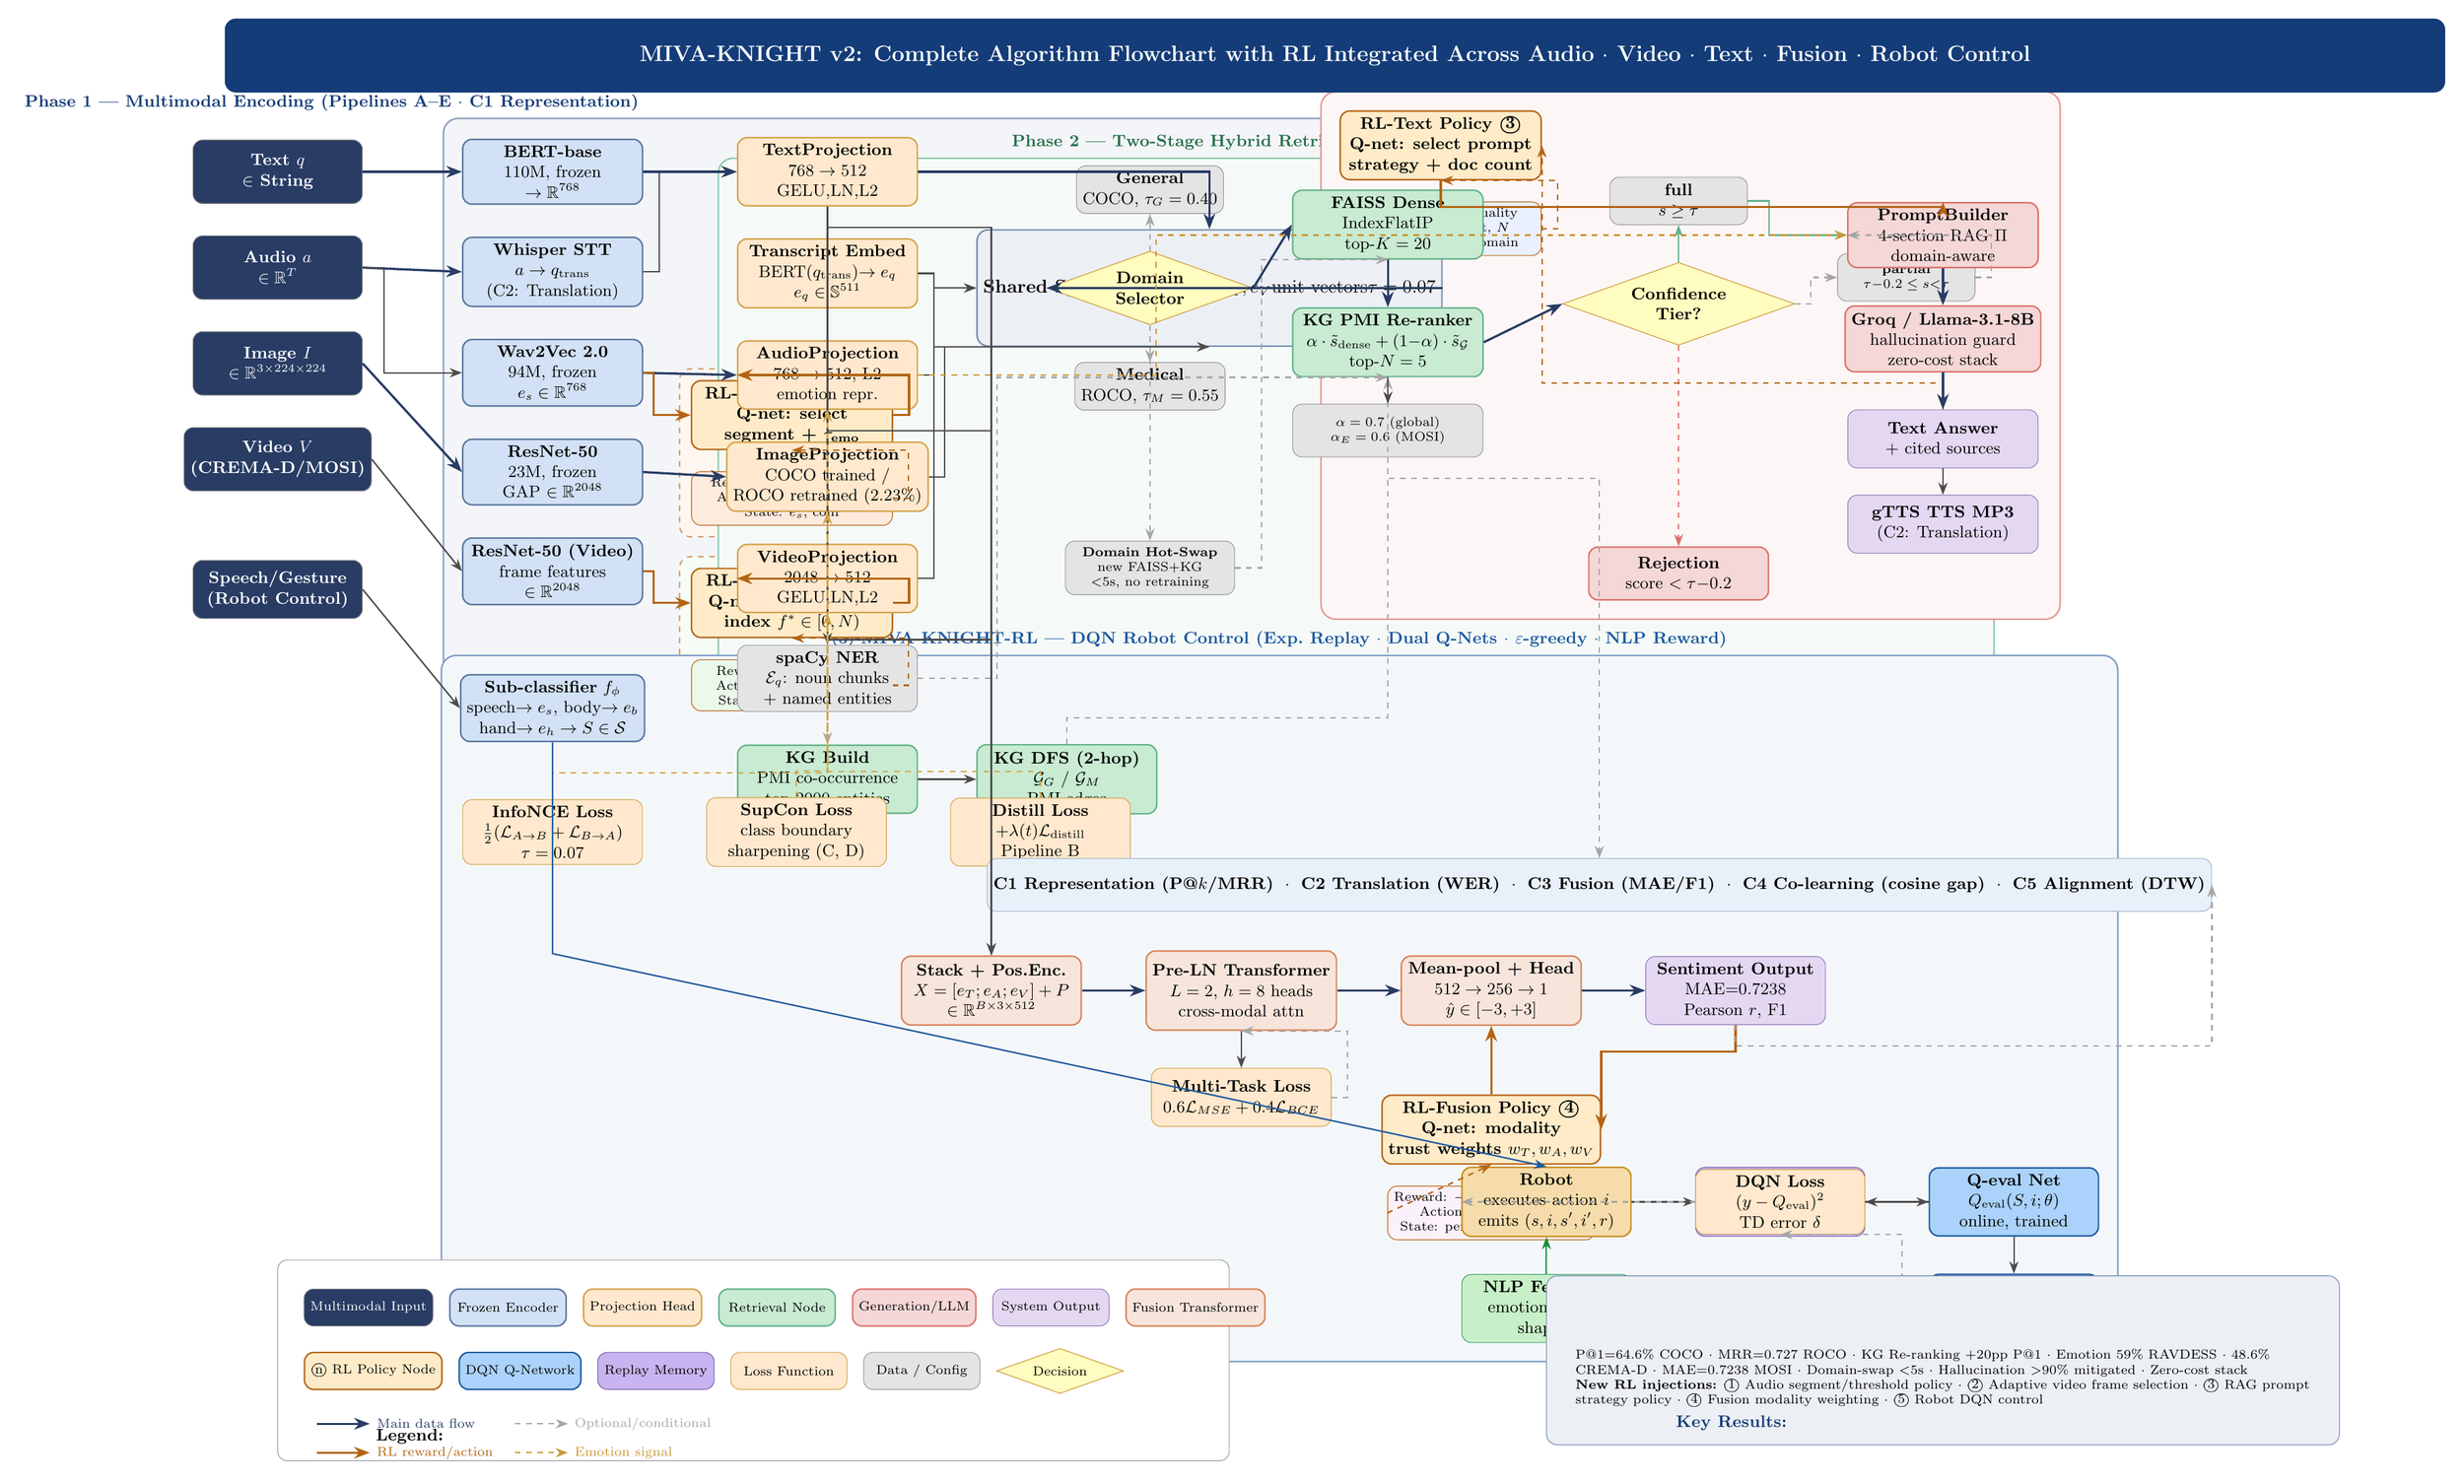
\begin{tikzpicture}[node distance=0.7cm and 1.2cm]

%%=============================================================
%% TITLE BANNER
%%=============================================================
\node[rectangle,fill=navyblue,text=white,font=\large\bfseries,
      minimum width=42cm,minimum height=1.4cm,rounded corners=6pt]
  (title) at (20,2.2)
  {MIVA-KNIGHT v2: Complete Algorithm Flowchart with RL Integrated Across Audio $\cdot$ Video $\cdot$ Text $\cdot$ Fusion $\cdot$ Robot Control};

%%=============================================================
%% COLUMN 1: MULTIMODAL INPUTS  (x≈0)
%%=============================================================
\node[inputnode,minimum width=3.2cm,minimum height=1.2cm]
  (textIn) at (0,0) {\textbf{Text} $q$\\$\in$ String};
\node[inputnode,minimum width=3.2cm,minimum height=1.2cm,below=0.6cm of textIn]
  (audioIn) {\textbf{Audio} $a$\\$\in\R^T$};
\node[inputnode,minimum width=3.2cm,minimum height=1.2cm,below=0.6cm of audioIn]
  (imageIn) {\textbf{Image} $I$\\$\in\R^{3\times224\times224}$};
\node[inputnode,minimum width=3.2cm,minimum height=1.2cm,below=0.6cm of imageIn]
  (vidIn) {\textbf{Video} $V$\\(CREMA-D/MOSI)};
\node[inputnode,minimum width=3.2cm,minimum height=1.1cm,below=1.3cm of vidIn]
  (gestIn) {\textbf{Speech/Gesture}\\(Robot Control)};

%%=============================================================
%% COLUMN 2: FROZEN ENCODERS  (x≈5.2)
%%=============================================================
\node[encnode,minimum width=3.4cm,minimum height=1.2cm]
  (bert) at (5.2,0) {\textbf{BERT-base}\\110M, frozen\\$\to\R^{768}$};
\node[encnode,minimum width=3.4cm,minimum height=1.2cm,below=0.6cm of bert]
  (whisper) {\textbf{Whisper STT}\\$a\to q_{\text{trans}}$\\(C2: Translation)};
\node[encnode,minimum width=3.4cm,minimum height=1.2cm,below=0.6cm of whisper]
  (w2v) {\textbf{Wav2Vec 2.0}\\94M, frozen\\$e_s\in\R^{768}$};
\node[encnode,minimum width=3.4cm,minimum height=1.2cm,below=0.6cm of w2v]
  (resnet) {\textbf{ResNet-50}\\23M, frozen\\GAP $\in\R^{2048}$};
\node[encnode,minimum width=3.4cm,minimum height=1.2cm,below=0.6cm of resnet]
  (resnetV) {\textbf{ResNet-50 (Video)}\\frame features\\$\in\R^{2048}$};
\node[encnode,minimum width=3.4cm,minimum height=1.2cm,below=1.3cm of resnetV]
  (subclf) {\textbf{Sub-classifier} $f_\phi$\\speech$\to e_s$, body$\to e_b$\\hand$\to e_h \to S\in\mathcal{S}$};

%%=============================================================
%% RL INJECTION 1: AUDIO — Adaptive Segment/Threshold Policy
%%=============================================================
\node[rlpnode,minimum width=3.8cm,minimum height=1.3cm,
      right=0.9cm of w2v,yshift=-0.8cm]
  (rlAudio) {\textbf{RL-Audio Policy} \textcircled{1}\\Q-net: select\\segment + $\tau_{\text{emo}}$};
% reward annotation
\node[datanode,fill=rlAudio!60,draw=rlpolicyborder,font=\scriptsize,
      below=0.4cm of rlAudio,minimum width=3.8cm]
  (rlAudioR) {Reward: correct emotion\\Action: segment choice\\State: $e_s$, conf};

%%=============================================================
%% RL INJECTION 2: VIDEO — Adaptive Frame Selection Policy
%%=============================================================
\node[rlpnode,minimum width=3.8cm,minimum height=1.3cm,
      right=0.9cm of resnetV,yshift=-0.6cm]
  (rlVideo) {\textbf{RL-Video Policy} \textcircled{2}\\Q-net: select frame\\index $f^* \in[0,N)$};
\node[datanode,fill=rlVideo!60,draw=rlpolicyborder,font=\scriptsize,
      below=0.4cm of rlVideo,minimum width=3.8cm]
  (rlVideoR) {Reward: class accuracy\\Action: frame index $f^*$\\State: ResNet features};

%%=============================================================
%% COLUMN 3: PROJECTION HEADS + NER  (x≈10.4)
%%=============================================================
\node[projnode,minimum width=3.4cm,minimum height=1.2cm]
  (tproj) at (10.4,0) {\textbf{TextProjection}\\$768\to512$\\GELU,LN,L2};
\node[projnode,minimum width=3.4cm,minimum height=1.2cm,below=0.6cm of tproj]
  (transOut) {\textbf{Transcript Embed}\\BERT($q_{\text{trans}}$)$\to e_q$\\$e_q\in\Sph^{511}$};
\node[projnode,minimum width=3.4cm,minimum height=1.2cm,below=0.6cm of transOut]
  (aproj) {\textbf{AudioProjection}\\$768\to512$, L2\\emotion repr.};
\node[projnode,minimum width=3.4cm,minimum height=1.2cm,below=0.6cm of aproj]
  (iproj) {\textbf{ImageProjection}\\COCO trained /\\ROCO retrained (2.23\%)};
\node[projnode,minimum width=3.4cm,minimum height=1.2cm,below=0.6cm of iproj]
  (vproj) {\textbf{VideoProjection}\\$2048\to512$\\GELU,LN,L2};
\node[datanode,minimum width=3.4cm,minimum height=1.1cm,below=0.6cm of vproj]
  (ner) {\textbf{spaCy NER}\\$\mathcal{E}_q$: noun chunks\\+ named entities};

%% Shared Embedding Space
\node[rectangle,draw=navyblue!60,fill=navyblue!8,rounded corners=6pt,thick,
      minimum width=3.6cm,minimum height=2.2cm,
      right=1.1cm of tproj,yshift=-2.2cm]
  (shared) {\textbf{Shared Space}\\\textbf{$\Sph^{511}$}\\$e_q,e_T,e_A,e_I,e_V$\\unit vectors\\$\tau=0.07$};

%%=============================================================
%% RL INJECTION 3: TEXT/PROMPT — RAG Prompt Strategy Policy
%%=============================================================
\node[rlpnode,minimum width=3.8cm,minimum height=1.3cm]
  (rlText) at (22.0, 0.5) {\textbf{RL-Text Policy} \textcircled{3}\\Q-net: select prompt\\strategy + doc count};
\node[datanode,fill=rlText!60,draw=rlpolicyborder,font=\scriptsize,
      below=0.4cm of rlText,minimum width=3.8cm]
  (rlTextR) {Reward: answer quality\\Action: $\Pi$ variant, $N$\\State: conf tier, domain};

%%=============================================================
%% DOMAIN ROUTING  (x≈16.5)
%%=============================================================
\node[decnode,minimum width=3.2cm]
  (dom) at (16.5,-2.2) {\textbf{Domain}\\Selector};
\node[datanode,minimum width=2.6cm,above=0.7cm of dom]
  (gdom) {\textbf{General}\\COCO, $\tau_G=0.40$};
\node[datanode,minimum width=2.6cm,below=0.7cm of dom]
  (mdom) {\textbf{Medical}\\ROCO, $\tau_M=0.55$};

%%=============================================================
%% KG CONSTRUCTION  (x≈10, y low)
%%=============================================================
\node[retnode,minimum width=3.4cm,minimum height=1.2cm]
  (kgbuild) at (10.4,-11.5) {\textbf{KG Build}\\PMI co-occurrence\\top-2000 entities};
\node[retnode,minimum width=3.4cm,minimum height=1.2cm,right=1.1cm of kgbuild]
  (kgdfs) {\textbf{KG DFS (2-hop)}\\$\mathcal{G}_G$ / $\mathcal{G}_M$\\PMI edges};

%%=============================================================
%% COLUMN 4: TWO-STAGE HYBRID RETRIEVAL  (x≈21)
%%=============================================================
\node[retnode,minimum width=3.6cm,minimum height=1.3cm]
  (faiss) at (21.0,-1.0) {\textbf{FAISS Dense}\\IndexFlatIP\\top-$K=20$};
\node[retnode,minimum width=3.6cm,minimum height=1.3cm,below=0.9cm of faiss]
  (kgrank) {\textbf{KG PMI Re-ranker}\\$\alpha\cdot\tilde{s}_{\text{dense}}+(1{-}\alpha)\cdot\tilde{s}_{\mathcal{G}}$\\top-$N=5$};
\node[datanode,minimum width=3.6cm,minimum height=1.0cm,below=0.5cm of kgrank,font=\scriptsize]
  (hybscore) {$\alpha=0.7$ (global)\\$\alpha_E=0.6$ (MOSI)};

%%=============================================================
%% COLUMN 5: TIERED CONFIDENCE  (x≈26.5)
%%=============================================================
\node[decnode,minimum width=3.4cm]
  (conf) at (26.5,-2.5) {\textbf{Confidence}\\Tier?};
\node[datanode,minimum width=2.6cm,above=0.7cm of conf]
  (full) {\textbf{full}\\$s\ge\tau$};
\node[datanode,minimum width=2.6cm,right=0.8cm of conf,yshift=0.5cm,font=\scriptsize]
  (partial) {\textbf{partial}\\$\tau{-}0.2\le s{<}\tau$};

%%=============================================================
%% COLUMN 6: RAG GENERATION  (x≈31.5)
%%=============================================================
\node[gennode,minimum width=3.6cm,minimum height=1.2cm]
  (prompt) at (31.5,-1.2) {\textbf{PromptBuilder}\\4-section RAG $\Pi$\\domain-aware};
\node[gennode,minimum width=3.6cm,minimum height=1.2cm,below=0.7cm of prompt]
  (llm) {\textbf{Groq / Llama-3.1-8B}\\hallucination guard\\zero-cost stack};
\node[outnode,minimum width=3.6cm,minimum height=1.1cm,below=0.7cm of llm]
  (textOut) {\textbf{Text Answer}\\+ cited sources};
\node[outnode,minimum width=3.6cm,minimum height=1.1cm,below=0.5cm of textOut]
  (tts) {\textbf{gTTS TTS MP3}\\(C2: Translation)};
\node[gennode,minimum width=3.4cm,minimum height=1.0cm,below=3.8cm of conf]
  (rej) {\textbf{Rejection}\\score $<\tau{-}0.2$};

%%=============================================================
%% HOT-SWAP
%%=============================================================
\node[datanode,minimum width=3.2cm,minimum height=1.0cm,font=\scriptsize]
  (swap) at (16.5,-7.5) {\textbf{Domain Hot-Swap}\\new FAISS+KG\\$<$5s, no retraining};

%%=============================================================
%% PIPELINE E: CROSS-MODAL FUSION TRANSFORMER  (y≈-15)
%%=============================================================
\node[fusnode,minimum width=3.4cm,minimum height=1.3cm]
  (stack) at (13.5,-15.5) {\textbf{Stack + Pos.Enc.}\\$X=[e_T;e_A;e_V]+P$\\$\in\R^{B\times3\times512}$};
\node[fusnode,minimum width=3.6cm,minimum height=1.5cm,right=1.2cm of stack]
  (transf) {\textbf{Pre-LN Transformer}\\$L=2$, $h=8$ heads\\cross-modal attn};
\node[fusnode,minimum width=3.4cm,minimum height=1.2cm,right=1.2cm of transf]
  (meanpool) {\textbf{Mean-pool + Head}\\$512\to256\to1$\\$\hat{y}\in[-3,+3]$};
\node[lossnode,minimum width=3.4cm,minimum height=1.1cm,below=0.7cm of transf]
  (eloss) {\textbf{Multi-Task Loss}\\$0.6\mathcal{L}_{MSE}+0.4\mathcal{L}_{BCE}$};
\node[outnode,minimum width=3.4cm,minimum height=1.1cm,right=1.2cm of meanpool]
  (sentOut) {\textbf{Sentiment Output}\\MAE=0.7238\\Pearson $r$, F1};

%%=============================================================
%% RL INJECTION 4: FUSION — Adaptive Modality Weighting Policy
%%=============================================================
\node[rlpnode,minimum width=3.8cm,minimum height=1.3cm,
      below=1.3cm of meanpool]
  (rlFusion) {\textbf{RL-Fusion Policy} \textcircled{4}\\Q-net: modality\\trust weights $w_T,w_A,w_V$};
\node[datanode,fill=rlFusion!40,draw=rlpolicyborder,font=\scriptsize,
      below=0.4cm of rlFusion,minimum width=3.8cm]
  (rlFusionR) {Reward: $-$MAE improvement\\Action: $(w_T,w_A,w_V)$\\State: per-modal confidence};

%%=============================================================
%% TRAINING LOSSES  (y≈-12)
%%=============================================================
\node[lossnode,minimum width=3.4cm,minimum height=1.2cm]
  (infonce) at (5.2,-12.5) {\textbf{InfoNCE Loss}\\$\frac{1}{2}(\mathcal{L}_{A\to B}+\mathcal{L}_{B\to A})$\\$\tau=0.07$};
\node[lossnode,minimum width=3.4cm,minimum height=1.2cm,right=1.2cm of infonce]
  (supcon) {\textbf{SupCon Loss}\\class boundary\\sharpening (C, D)};
\node[lossnode,minimum width=3.4cm,minimum height=1.2cm,right=1.2cm of supcon]
  (distill) {\textbf{Distill Loss}\\$+\lambda(t)\mathcal{L}_{\text{distill}}$\\Pipeline B};

%%=============================================================
%% RL EXTENSION 5: ROBOT CONTROL  (y≈-19, right side)
%%=============================================================
\node[robotnode,minimum width=3.2cm,minimum height=1.2cm]
  (robot) at (24.0,-19.5) {\textbf{Robot}\\executes action $i$\\emits $(s,i,s',i',r)$};
\node[memnode,minimum width=3.2cm,minimum height=1.2cm,right=1.2cm of robot]
  (memory) {\textbf{Replay Memory}\\ring-buffer\\push / sample};
\node[qnetnode,minimum width=3.2cm,minimum height=1.2cm,right=1.2cm of memory]
  (qeval) {\textbf{Q-eval Net}\\$Q_{\text{eval}}(S,i;\theta)$\\online, trained};
\node[qnetnode,minimum width=3.2cm,minimum height=1.2cm,below=0.7cm of qeval]
  (qtgt) {\textbf{Q-target Net}\\$Q_{\text{tgt}}(S,i;\theta^-)$\\frozen, sync every $C$};
\node[lossnode,minimum width=3.2cm,minimum height=1.1cm,left=1.2cm of qeval]
  (dqnloss) {\textbf{DQN Loss}\\$(y-Q_{\text{eval}})^2$\\TD error $\delta$};
\node[nlpnode,minimum width=3.2cm,minimum height=1.1cm,below=0.7cm of robot]
  (nlp) {\textbf{NLP Feedback}\\emotion reward\\shaping};

%%=============================================================
%% FIVE CHALLENGE BANNER
%%=============================================================
\node[basebox,fill=boxblue!50,draw=navyblue!40,minimum width=22.0cm,minimum height=1.0cm,
      font=\small\bfseries]
  (challenges) at (25.0,-13.5)
  {C1 Representation (P@$k$/MRR) $\;\cdot\;$
   C2 Translation (WER) $\;\cdot\;$
   C3 Fusion (MAE/F1) $\;\cdot\;$
   C4 Co-learning (cosine gap) $\;\cdot\;$
   C5 Alignment (DTW)};

%%=============================================================
%% CONNECTIONS — Input → Encoders
%%=============================================================
\draw[thickarr] (textIn.east) -- (bert.west);
\draw[thickarr] (audioIn.east) -- (whisper.west);
\draw[arr] (audioIn.east) -- ++(0.4,0) |- (w2v.west);
\draw[thickarr] (imageIn.east) -- (resnet.west);
\draw[arr] (vidIn.east) -- (resnetV.west);
\draw[arr] (gestIn.east) -- (subclf.west);

%% Whisper → BERT
\draw[arr] (whisper.east) -- ++(0.3,0) |- (tproj.west);

%% Encoders → Projections
\draw[thickarr] (bert.east) -- (tproj.west);
\draw[thickarr] (w2v.east) -- (aproj.west);
\draw[thickarr] (resnet.east) -- (iproj.west);

%% RL-Audio: Wav2Vec → RL policy → AudioProj
\draw[rlarr] (w2v.east) -- ++(0.2,0) |- (rlAudio.west);
\draw[rlarr] (rlAudio.east) -- ++(0.3,0) |- (aproj.west);
\draw[rldasharr] (rlAudioR.east) -- ++(0.3,0) |- (rlAudio.south);

%% RL-Video: ResNetV → RL policy → VideoProj
\draw[rlarr] (resnetV.east) -- ++(0.2,0) |- (rlVideo.west);
\draw[rlarr] (rlVideo.east) -- ++(0.3,0) |- (vproj.west);
\draw[rldasharr] (rlVideoR.east) -- ++(0.3,0) |- (rlVideo.south);

%% Projections → Shared space
\draw[thickarr] (tproj.east) -| (shared.north);
\draw[arr] (transOut.east) -- ++(0.3,0) |- (shared.west);
\draw[arr] (aproj.east) -- ++(0.3,0) |- (shared.west);
\draw[arr] (iproj.east) -- ++(0.3,0) |- (shared.south);
\draw[arr] (vproj.east) -- ++(0.3,0) |- (shared.south);

%% NER
\draw[arr] (tproj.south) -- (ner.north);

%% Shared → Domain
\draw[thickarr] (shared.east) -- (dom.west);

%% Domain routing
\draw[dasharr] (dom.north) -- (gdom.south);
\draw[dasharr] (dom.south) -- (mdom.north);

%% Domain → FAISS
\draw[thickarr] (dom.east) -- (faiss.west);

%% KG
\draw[arr] (kgbuild.east) -- (kgdfs.west);
\draw[dasharr] (kgdfs.north) -- ++(0,0.5) -| (kgrank.south);
\draw[dasharr] (ner.south) -- ++(0,-0.4) -| (kgbuild.north);
\draw[dasharr] (ner.east) -- ++(1.5,0) |- (kgrank.south);

%% FAISS → KG Reranker
\draw[thickarr] (faiss.south) -- (kgrank.north);
\draw[arr] (kgrank.south) -- (hybscore.north);

%% KG Reranker → Confidence
\draw[thickarr] (kgrank.east) -- (conf.west);

%% Confidence → Prompt/Rejection
\draw[arr,color=mintgreen!80] (conf.north) -- (full.south);
\draw[arr,color=mintgreen!80] (full.east) -- ++(0.4,0) |- (prompt.west);
\draw[dasharr] (conf.east) -- ++(0.3,0) |- (partial.west);
\draw[dasharr] (partial.east) -- ++(0.3,0) |- (prompt.west);
\draw[redarr,dashed] (conf.south) -- (rej.north);

%% RL-Text policy → PromptBuilder
\draw[rlarr] (rlText.south) -- ++(0,-0.5) -| (prompt.north);
\draw[rldasharr] (rlTextR.east) -- ++(0.3,0) |- (rlText.south);
%% feedback from LLM output quality → RL-Text reward
\draw[rldasharr,bend left=20] (textOut.north) -- ++(0,0.5) -| (rlText.east);

%% RAG chain
\draw[thickarr] (prompt.south) -- (llm.north);
\draw[thickarr] (llm.south) -- (textOut.north);
\draw[arr] (textOut.south) -- (tts.north);

%% Emotion → PromptBuilder
\draw[ambarr] (aproj.east) -- ++(4.5,0) |- (prompt.west);

%% Hot-swap
\draw[dasharr] (dom.south) -- ++(0,-1.5) -- (swap.north);
\draw[dasharr] (swap.east) -- ++(0.5,0) |- (faiss.south);

%% Pipeline E connections
\draw[arr] (vproj.south) -- ++(0,-0.5) -| (stack.north);
\draw[arr] (aproj.south) -- ++(0,-0.4) -| (stack.north);
\draw[arr] (tproj.south) -- ++(0,-0.4) -| (stack.north);
\draw[thickarr] (stack.east) -- (transf.west);
\draw[thickarr] (transf.east) -- (meanpool.west);
\draw[arr] (transf.south) -- (eloss.north);
\draw[thickarr] (meanpool.east) -- (sentOut.west);
\draw[dasharr] (eloss.east) -- ++(0.3,0) |- (transf.south);

%% RL-Fusion: feedback from MAE → policy → modality weights
\draw[rlarr] (sentOut.south) -- ++(0,-0.5) -| (rlFusion.east);
\draw[rlarr] (rlFusion.north) -- ++(0,0.5) -| (meanpool.south);
\draw[rldasharr] (rlFusionR.west) -- (rlFusion.south);

%% Training losses ↔ projections
\draw[dasharr,color=amber!80] (infonce.north) -- ++(0,0.5) -| (aproj.south);
\draw[dasharr,color=amber!80] (infonce.north) -- ++(0,0.5) -| (iproj.south);
\draw[dasharr,color=amber!80] (supcon.north) -- ++(0,0.5) -| (vproj.south);
\draw[dasharr,color=amber!80] (distill.north) -- ++(0,0.5) -| (iproj.south);

%% Challenges banner
\draw[dasharr] (hybscore.south) -- ++(0,-0.4) -| (challenges.north);
\draw[dasharr] (sentOut.south) -- ++(0,-0.4) -| (challenges.east);

%% RL Robot loop
\draw[bluearr] (subclf.south) -- ++(0,-4.0) -- (robot.north);
\draw[arr] (robot.east) -- (memory.west);
\draw[arr] (memory.east) -- (qeval.west);
\draw[arr] (qeval.south) -- (qtgt.north);
\draw[arr] (qeval.west) -- (dqnloss.east);
\draw[dasharr] (dqnloss.west) -- ++(-.4,0) |- (robot.west);
\draw[arr,color=rlgreen] (nlp.north) -- (robot.south);
\draw[dasharr] (qtgt.west) -- ++(-0.5,0) |- (dqnloss.south);

%%=============================================================
%% PHASE BACKGROUND BOXES
%%=============================================================
\begin{pgfonlayer}{background}

%% Phase 1 — Encoding
\node[rectangle,draw=navyblue!50,fill=navyblue!5,rounded corners=8pt,thick,
      fit=(bert)(whisper)(w2v)(resnet)(resnetV)
          (tproj)(transOut)(aproj)(iproj)(vproj)(ner)(shared),
      inner sep=10pt,
      label={[font=\small\bfseries,color=navyblue]above left:
        \textbf{Phase 1 — Multimodal Encoding} (Pipelines A–E $\cdot$ C1 Representation)}] {};

%% RL-Audio zone
\node[rectangle,draw=rlpolicyborder!60,fill=rlAudio!25,rounded corners=6pt,dashed,thick,
      fit=(rlAudio)(rlAudioR),inner sep=6pt,
      label={[font=\scriptsize\bfseries,color=rlpolicyborder]above:
        \textcircled{1} RL-Audio}] {};

%% RL-Video zone
\node[rectangle,draw=rlpolicyborder!60,fill=rlVideo!25,rounded corners=6pt,dashed,thick,
      fit=(rlVideo)(rlVideoR),inner sep=6pt,
      label={[font=\scriptsize\bfseries,color=rlpolicyborder]above:
        \textcircled{2} RL-Video}] {};

%% Phase 2 — Retrieval
\node[rectangle,draw=mintgreen!60,fill=mintgreen!5,rounded corners=8pt,thick,
      fit=(faiss)(kgrank)(hybscore)(conf)(full)(partial)(kgbuild)(kgdfs),
      inner sep=10pt,
      label={[font=\small\bfseries,color=mintgreen!70!black]above:
        \textbf{Phase 2 — Two-Stage Hybrid Retrieval} (Dense FAISS + KG PMI Re-ranking)}] {};

%% Phase 3 — Generation + RL-Text
\node[rectangle,draw=coralred!60,fill=coralred!5,rounded corners=8pt,thick,
      fit=(prompt)(llm)(textOut)(tts)(rej)(rlText)(rlTextR),
      inner sep=10pt,
      label={[font=\small\bfseries,color=coralred]above:
        \textbf{Phase 3 — RAG Generation + \textcircled{3} RL-Text Prompt Policy}
        ($\cdot$ Tiered Confidence $\cdot$ C2 Translation)}] {};

%% Pipeline E Fusion box
\node[rectangle,draw=fusioncolor!60,fill=fusioncolor!5,rounded corners=8pt,thick,
      fit=(stack)(transf)(meanpool)(eloss)(sentOut)(rlFusion)(rlFusionR),
      inner sep=10pt,
      label={[font=\small\bfseries,color=fusioncolor]above:
        \textbf{Pipeline E — Cross-Modal Fusion Transformer + \textcircled{4} RL-Fusion Weighting}
        ($\cdot$ C3 Fusion $\cdot$ CMU-MOSI $\cdot$ MAE=0.7238)}] {};

%% Training Losses box
\node[rectangle,draw=amber!60,fill=amber!5,rounded corners=8pt,thick,
      fit=(infonce)(supcon)(distill),inner sep=8pt,
      label={[font=\small\bfseries,color=amber!80!black]above:
        \textbf{Contrastive Training} (InfoNCE + SupCon + Distillation $\cdot$ Pipelines A–D)}] {};

%% RL Robot box
\node[rectangle,draw=rlblue!60,fill=rlblue!5,rounded corners=8pt,thick,
      fit=(robot)(memory)(qeval)(qtgt)(dqnloss)(nlp)(subclf),
      inner sep=10pt,
      label={[font=\small\bfseries,color=rlblue]above:
        \textcircled{5} \textbf{MIVA-KNIGHT-RL — DQN Robot Control}
        (Exp.\ Replay $\cdot$ Dual Q-Nets $\cdot$ $\varepsilon$-greedy $\cdot$ NLP Reward)}] {};

\end{pgfonlayer}

%%=============================================================
%% LEGEND
%%=============================================================
\node[rectangle,draw=black!40,fill=white,rounded corners=5pt,
      minimum width=18cm,minimum height=3.8cm]
  (legend) at (9.0,-22.5) {};

\node[font=\small\bfseries,above=0.2cm of legend.south,xshift=-6.5cm] {Legend:};

\node[inputnode,minimum width=2.2cm,minimum height=0.7cm,font=\scriptsize,
      right=0.5cm of legend.west,yshift=1.0cm] (lg1) {Multimodal Input};
\node[encnode,minimum width=2.2cm,minimum height=0.7cm,font=\scriptsize,
      right=0.3cm of lg1] (lg2) {Frozen Encoder};
\node[projnode,minimum width=2.2cm,minimum height=0.7cm,font=\scriptsize,
      right=0.3cm of lg2] (lg3) {Projection Head};
\node[retnode,minimum width=2.2cm,minimum height=0.7cm,font=\scriptsize,
      right=0.3cm of lg3] (lg4) {Retrieval Node};
\node[gennode,minimum width=2.2cm,minimum height=0.7cm,font=\scriptsize,
      right=0.3cm of lg4] (lg5) {Generation/LLM};
\node[outnode,minimum width=2.2cm,minimum height=0.7cm,font=\scriptsize,
      right=0.3cm of lg5] (lg6) {System Output};
\node[fusnode,minimum width=2.2cm,minimum height=0.7cm,font=\scriptsize,
      right=0.3cm of lg6] (lg7) {Fusion Transformer};

\node[rlpnode,minimum width=2.6cm,minimum height=0.7cm,font=\scriptsize,
      right=0.5cm of legend.west,yshift=-0.2cm] (lg8) {\textcircled{n} RL Policy Node};
\node[qnetnode,minimum width=2.2cm,minimum height=0.7cm,font=\scriptsize,
      right=0.3cm of lg8] (lg9) {DQN Q-Network};
\node[memnode,minimum width=2.2cm,minimum height=0.7cm,font=\scriptsize,
      right=0.3cm of lg9] (lg10) {Replay Memory};
\node[lossnode,minimum width=2.2cm,minimum height=0.7cm,font=\scriptsize,
      right=0.3cm of lg10] (lg11) {Loss Function};
\node[datanode,minimum width=2.2cm,minimum height=0.7cm,font=\scriptsize,
      right=0.3cm of lg11] (lg12) {Data / Config};
\node[decnode,minimum width=2.4cm,minimum height=0.7cm,font=\scriptsize,
      right=0.3cm of lg12] (lg13) {Decision};

%% Arrow legend
\node[right=0.5cm of legend.west,yshift=-1.2cm,font=\scriptsize] (ala) {};
\draw[thickarr] (ala.east) -- ++(1.0,0) node[right,font=\scriptsize] {Main data flow};
\node[below=0.3cm of ala,font=\scriptsize] (alb) {};
\draw[rlarr] ([xshift=0.0cm]alb.east) -- ++(1.0,0) node[right,font=\scriptsize] {RL reward/action};
\node[right=3.5cm of ala,font=\scriptsize] (alc) {};
\draw[dasharr] (alc.east) -- ++(1.0,0) node[right,font=\scriptsize] {Optional/conditional};
\node[right=3.5cm of alb,font=\scriptsize] (ald) {};
\draw[ambarr] (ald.east) -- ++(1.0,0) node[right,font=\scriptsize] {Emotion signal};

%%=============================================================
%% RESULTS BADGE
%%=============================================================
\node[rectangle,draw=navyblue!60,fill=navyblue!8,rounded corners=6pt,
      minimum width=15cm,minimum height=3.2cm]
  (results) at (31.5,-22.5) {};
\node[font=\small\bfseries,color=navyblue,
      above=0.15cm of results.south,xshift=-4cm] {Key Results:};
\node[font=\scriptsize,above=0.6cm of results.south,text width=14.5cm,align=flush left,xshift=0.3cm]
  {P@1=64.6\% COCO $\cdot$ MRR=0.727 ROCO $\cdot$ KG Re-ranking +20pp P@1
   $\cdot$ Emotion 59\% RAVDESS $\cdot$ 48.6\% CREMA-D
   $\cdot$ MAE=0.7238 MOSI $\cdot$ Domain-swap $<$5s
   $\cdot$ Hallucination $>$90\% mitigated $\cdot$ Zero-cost stack\\
   \textbf{New RL injections:}
   \textcircled{1} Audio segment/threshold policy
   $\cdot$ \textcircled{2} Adaptive video frame selection
   $\cdot$ \textcircled{3} RAG prompt strategy policy
   $\cdot$ \textcircled{4} Fusion modality weighting
   $\cdot$ \textcircled{5} Robot DQN control};

\end{tikzpicture}
\end{document}
